\begin{frame}
    \frametitle{Representación de Posición del Robot 2D}

\end{frame}


\begin{frame}
    \frametitle{Right-hand rule}
    En Robótica la disposición de los ejes de coordenadas y el sentido de rotación de los mismos está dado por la regla de la mano derecha (Right-hand rule).
    
    \begin{figure}[!h]
        \centering
        \subfloat[]
        {
            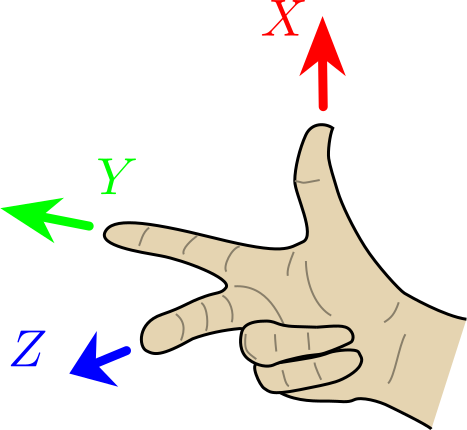
\includegraphics[width=0.4\columnwidth]{./images/right_hand_rule.pdf}
        }\hfill
        \subfloat[]
        {
            
\includegraphics[width=0.4\columnwidth]{./images/right_hand_rule_positive_rotation.pdf}
        }
    \end{figure}
\end{frame}

\begin{frame}
    \frametitle{Roll Pitch Yaw }
        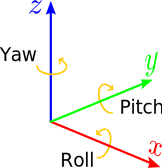
\includegraphics[width=0.5\columnwidth]{./images/roll_pitch_yaw.pdf}
        
        \TODO{Gimbal-Lock Video explanation: https://youtu.be/-WXfEPg8eMM}
\end{frame}
       
\begin{frame}
    \frametitle{Left-hand vs Right-hand rule}
    \begin{center}
        \only<1>{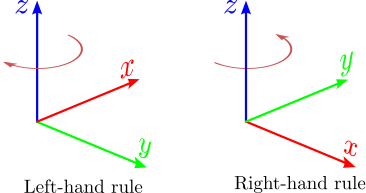
\includegraphics[width=\columnwidth]{./images/left_right_hand_rule.pdf}}
        \only<2>{\includegraphics[width=\columnwidth]{./images/left_right_hand_rule_cross.pdf}}
    \end{center}
\end{frame}

\begin{frame}
    \frametitle{Sistema de referencia Local y Global}
    Poner imagen 3.1 del libro
\end{frame}